\documentclass[conf]{new-aiaa}
%\documentclass[journal]{new-aiaa} for journal papers
\usepackage[utf8]{inputenc}
\usepackage{listings}
\usepackage{graphicx}
\usepackage{amsmath}
\usepackage[version=4]{mhchem}
\usepackage{siunitx}
\usepackage{longtable,tabularx}
\usepackage{float}
\usepackage{pdfpages}
\setlength\LTleft{0pt}


\title{Sound and Light Propagation}
\author{Liam Nestelroad \footnote{ID: 108020371}}

\begin{document}

\begin{titlepage}

\newcommand{\HRule}{\rule{\linewidth}{0.5mm}}

\center
 
\textsc{\LARGE University of Colorado - Boulder}\\[1.5cm]
\textsc{\Large <CLASS NAME>}\\[0.5cm] % Major heading such as course name
\textsc{\large <ASSIGNMENT TITLE>}\\[0.5cm] % Minor heading such as course title

\HRule \\[0.4cm]
{ \huge \bfseries <PAPER TITLE>}\\[0.4cm] 
\HRule \\[1.5cm]

\begin{figure}[H]
    \centering
    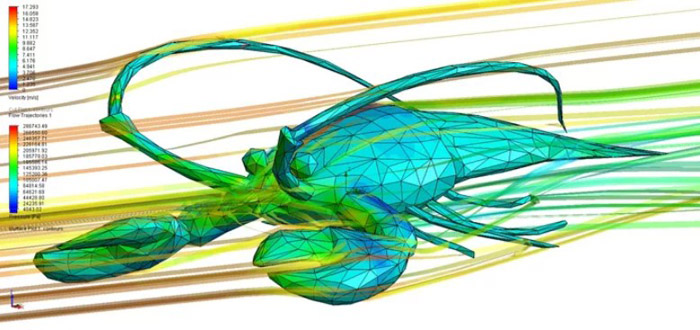
\includegraphics[width=0.65\textwidth]{template_image.jpeg}
\end{figure}



\begin{minipage}{0.4\textwidth}
\begin{flushleft} \large
\emph{Author:}\\
Liam \textsc{Nestelroad} 
\end{flushleft}
\end{minipage}
~
\begin{minipage}{0.4\textwidth}
\begin{flushright} \large
\emph{Professor:} \\
Dr. \textsc{Bhat} 
\end{flushright}
\end{minipage}\\[1cm]

{\large January 1, 1970}\\[2cm] 
 
\vfill

\end{titlepage}

\newpage
\renewcommand\contentsname{Table of Contents}
\doublespacing
\tableofcontents
\singlespacing
\addtocontents{toc}{~\hfill\textbf{Page}\par}
\newpage

\maketitle
\begin{abstract}

\end{abstract}

\newpage




\section{Abstract}

\section{Body}

\section{Conclusion}

\section{Acknowledgements}
\newpage

\begin{thebibliography}{}

\bibitem{baker} Baker, N. 1966,
    in Stellar Evolution,
    ed.\ R. F. Stein \& A. G. W. Cameron
    (Plenum, New York) 333

\end{thebibliography}

\newpage
\end{document}